The virial theorem tells us the relation between expectation values of kinetic $<T>$ and potential energy $<V>$.
For two special interactions, H.O. potential and Coulomb repulsion.
The relations are
\begin{equation}\label{eq:virial}
	<T>=<V>\ (\rm{H.O.})
\end{equation}
\begin{equation}
	<T>=\frac{1}{2}<V>\ (\rm{Coulomb})
\end{equation}
Both these two interactions exist in our system, so the ratio between $<T>$ and $<V>$, where we defined as $\chi$ should locates between 0.5 and 1.
The $\chi$ value is determined by relative strength between these two interactions.

In our calculations, we consider two situations using 
the first trail wave function $\Phi_{t1}$.
One without Coulomb interaction then $\alpha=1.0$, as expected, because it's a product of two free electrons' wave functions.
The other with Coulomb interaction has different value of optimal $\alpha$ for different  $\omega$. 
We vary $\omega \in [0.01,1]$ to control relative strength between H.O. potential and Coulomb repulsion and calculate the value of $\chi$.
\begin{figure}[tb]
\label{fig:virial}
\centering
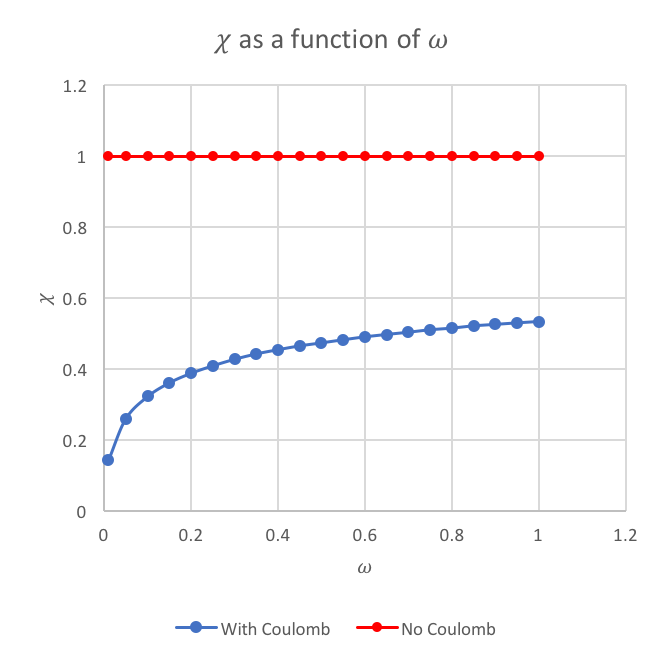
\includegraphics[width=0.4\textwidth]{virial.png}
\caption{Relation between lowest $E$(a.u.) and the variational parameters $\alpha$ and $\beta$ where $\omega$ is set to one and $N=10^7$ obtained from $\Phi_{t2}$.}
\end{figure}
The results are shown in Fig. \ref{fig:virial}.
The red curve is the one without Coulomb repulsion.
It gives a trivial result follows Eqt. \ref{eq:virial}.
For the blue curve represents situation with Coulomb repulsion.
As expected, We can see $\chi$ growths with increasing $\omega$ which indicates stronger H.O. potentials.
However, its value doesn't locate in 0.5 and 1. 
My suggestion for this problem is on trail wave function $\Phi_{t1}$ we used.
It has a form of free electron in H.O. potential, so it deviates a lot from exact one especially for weak H.O. potentials (small $\omega$).
